\documentclass[12pt]{article}
\usepackage{packages}

\begin{document}
\begin{figure*}
    \centering 
    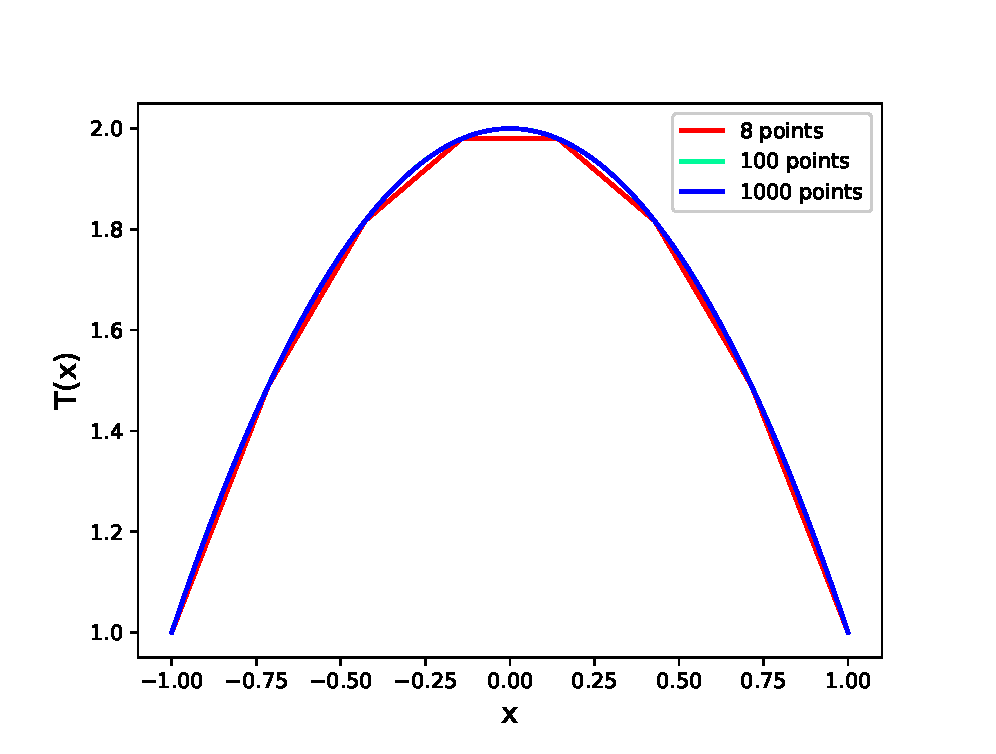
\includegraphics[width=\textwidth]{gauss.eps}
    \caption{Forward elimination - backward substitution (Gauss-Jordan) for $N=8, 100, 1000$ gridpoints}
\end{figure*}
\begin{figure*}
    \centering 
    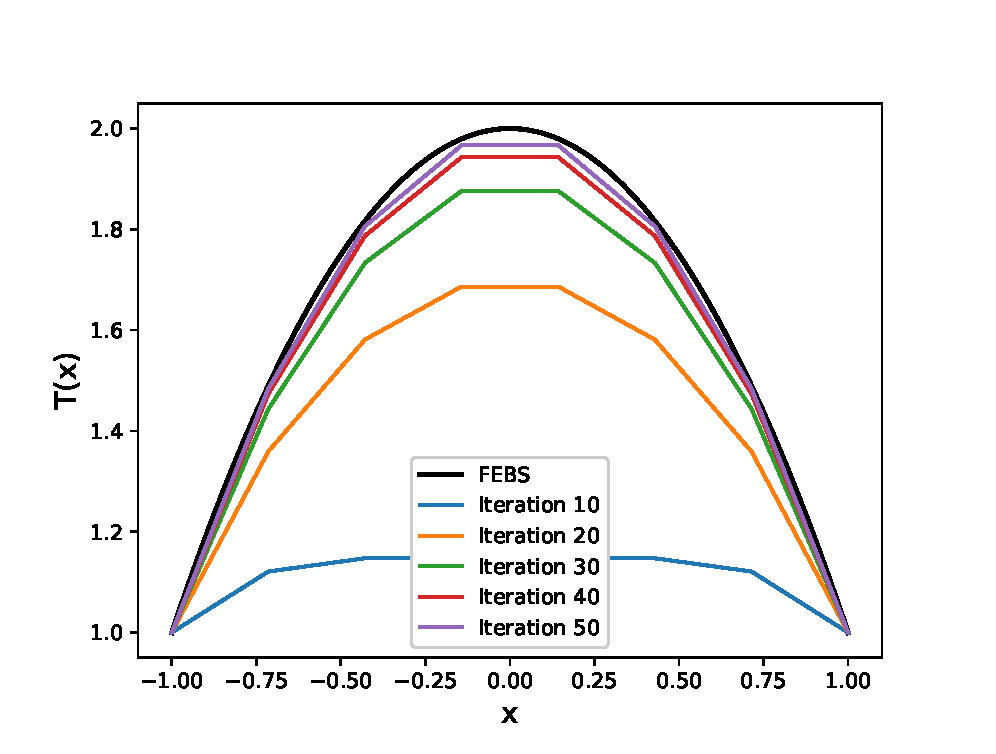
\includegraphics[width=\textwidth]{jacobi8.eps}
    \caption{Comparison between the forward elimination - backward substitution method for $N=1000$ gridpoints and $50$ Jacobi iterations with $N=8$ gridpoints}
\end{figure*}
\begin{figure*}
    \centering 
    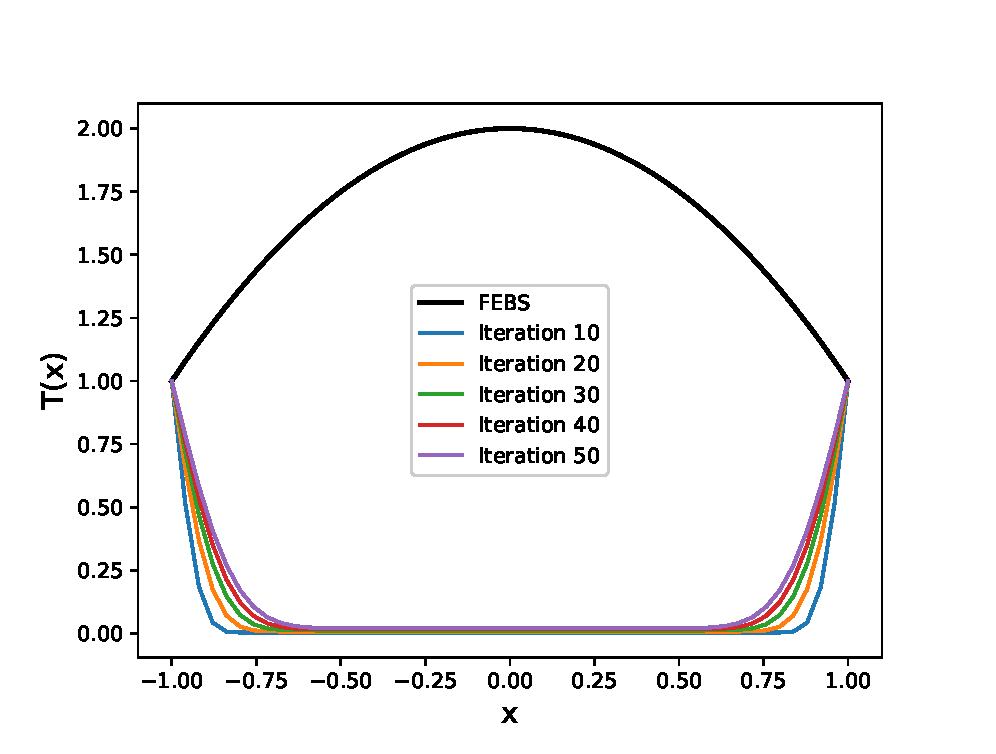
\includegraphics[width=\textwidth]{jacobi100.eps}
    \caption{Comparison between the forward elimination - backward substitution method for $N=1000$ gridpoints and $50$ Jacobi iterations with $N=100$ gridpoints}
\end{figure*}
\end{document}